\documentclass{article}
\usepackage{qilin}
\tikzstyle{process} = [rectangle, rounded corners, minimum width=1.5cm, minimum height=0.5cm,align=center, draw=black, fill=gray!30, auto]
\title{MAT257: Real Analysis II}
\author{QiLin Xue}
\date{Fall 2021}
\usepackage{mathrsfs}
\usetikzlibrary{arrows}
\usepackage{stmaryrd}

\begin{document}

\maketitle
\tableofcontents
\newpage
\section{Introduction}
\textit{Covers 1.1: Mathematical Models and Solutions}
\begin{itemize}
    \item Big Idea: Differential equations model physical situations:
          \begin{itemize}
              \item Take a physical situation and ODE-ify it (How do we model a cooling coffee cup?)
              \item Understand an ODE without solving it (What can we deduce directly from $y'=y^2$?)
              \item Study, categories, typecast ODEs and solve them
                    \begin{example}
                        Suppose we have $y'=y/t+\ln t$ and $y'=y^2+t$. Which of these are harder to solve (without actually solving them)?
                        \vspace{2mm}

                        It turns out that the second one is harder as it is \textit{non-linear}.
                    \end{example}
              \item Handle ODEs numerically (What do we do when we cannot solve an ODE that models a real life phenomenon?)
              \item The art of problem solving (How do I work with no strings attached?)
          \end{itemize}
    \item What is a differential equation?
          \begin{definition}
              A differential equation relates a function and its derivatives.
          \end{definition}
    \item We can understand ODEs without solving it:
          \begin{example}
              Let's consider a cup of coffee in a room. We want to model its change in temperature over time. How do we do this?
              \vspace{2mm}

              There are a lot of variables, so we have to simplify our model. The things we care about
              \begin{itemize}
                  \item The temperature of the coffee cup $y(t)$.
                  \item $t$ is in minutes.
                  \item $y(t)$ is in Celsius.
                  \item The temperature in the room $T$ (in Celsius).
              \end{itemize}
              The things we ignore / simplify:
              \begin{itemize}
                  \item Temperature variation within the cup
                  \item Temperature variation in the room
              \end{itemize}
              \textbf{Exercise:} Let's consider some suggestions for an ODE describing the temperature of a coffee cup in a room. Each of the following suggested ODEs contradicts our intuition in some way. How?

              \begin{itemize}
                  \item $y'=y^2$
                        \begin{itemize}
                            \item $T$ isn't in there
                            \item Temperature would always increase except if $y=0$.
                            \item The hotter the coffee, the faster it heats up.
                        \end{itemize}
                  \item $y'=\frac{T}{y}$
                        \begin{itemize}
                            \item If $T>0, y>0$, then $y'>0$
                            \item The model doesn't work for coffee at $0^\circ \text{C}$.
                        \end{itemize}
                  \item $y'=y[e^{y-T}+y^3]$
                  \item $y'=y-T$
                  \item $y'=T-y$
                        \begin{itemize}
                            \item There should be a parameter that describes the physical properties (rate of heating/cooling will be different for different materials)
                        \end{itemize}
              \end{itemize}
          \end{example}
          \begin{idea}
              Without solving an ODE, you can already make many predictions about its solution
              \vspace{2mm}

              (and then, for example, judge your model)
          \end{idea}
    \item We introduce a few definitions
          \begin{definition}
              An \textbf{ordinary differential equation} (ODE) only considers a function of $1$ variable and its derivatives
          \end{definition}
          \begin{definition}
              A \textbf{partial differential equation} considers a function of several variables and its derivatives.
          \end{definition}
    \item The most general ODE for a function $y(t)$ is:
          \begin{enumerate}[label=(\alph*)]
              \item $F[t,y,y'',\dots,y^{(n)}]$ for $n\in \mathbb{N}$.
              \item Any function that satisfies this equation is called \textit{a solution}
          \end{enumerate}
          \begin{definition}
              The order of an ODE is the highest derivative of an ODE.
          \end{definition}
    \item An autonomous ODE is if the independent variable doesn't appear in the ODE.
    \item Systems of ODEs arise if we study several quantities depending on the same variable and how their changes interact.
          \begin{example}
              Assume that $p(t)$ and $o(t)$ describe the number of twitter followers of two accounts. If there is no interaction, what are reasonable ODEs for these two quantities?
              \begin{align}
                  p'(t) = kp(t) \\
                  o'(t) = \ell o(t)
              \end{align}
              Suppose that if in addition to ``word of mouth,'' we consider the effects that these two tweets have, what are reasonable ODEs for the number of followers?
              \begin{align}
                  p'(t) = k \cdot p(t) - m \cdot o(t) \\
                  o'(t) = \ell \cdot o(t) - n \cdot p(t)
              \end{align}
              where all constant are positive. However, this is oversimplified as it assumes the people who follow \textit{O} also follow \textit{P.}
          \end{example}
    \item Suppose a differential equation is given by
          \begin{equation}
              y'(t) = -1.5(y(t)-1)
          \end{equation}
          \begin{definition}
              Consider the ODE $y'=f(t,y)$. We can draw a \textbf{direction field} as follows:
              \begin{enumerate}
                  \item Draw a $t-y$ coordinate system.
                  \item Evaluate $f(t,y)$ over a rectangular grid of points.
                  \item Draw a line at each point $(t,y)$ of the grid with slope $f(t,y)$.
              \end{enumerate}
          \end{definition}
          \begin{center}
              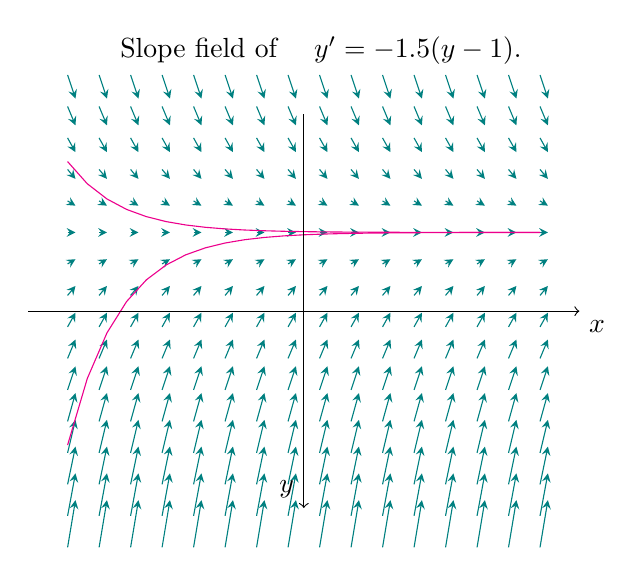
\begin{tikzpicture}[declare function={f(\x,\y)=-1.5*(\y-1);}]
                  \def\xmax{3} \def\xmin{-3}
                  \def\ymax{-3} \def\ymin{3}
                  \def\nx{15}  \def\ny{15}

                  \pgfmathsetmacro{\hx}{(\xmax-\xmin)/\nx}
                  \pgfmathsetmacro{\hy}{(\ymax-\ymin)/\ny}
                  \foreach \i in {0,...,\nx}
                  \foreach \j in {0,...,\ny}{
                          \pgfmathsetmacro{\yprime}{f({\xmin+\i*\hx},{\ymin+\j*\hy})}
                          \draw[teal,-stealth,shift={({\xmin+\i*\hx},{\ymin+\j*\hy})}] (0,0)--(.1,.1*\yprime);
                      }

                  % a solution y=(yo+1)e^x-x-1
                  \def\yo{0.01}
                  \def\yoo{-0.03}
                  \draw[magenta] plot[domain=\xmin:\xmax] (\x,{(\yo)*exp(-1.5*\x)+1});
                  \draw[magenta] plot[domain=\xmin:\xmax] (\x,{(\yoo)*exp(-1.5*\x)+1});

                  \draw[->] (\xmin-.5,0)--(\xmax+.5,0) node[below right] {$x$};
                  \draw[->] (0,\ymin-.5)--(0,\ymax+.5) node[above left] {$y$};
                  \draw (current bounding box.north) node[above]
                  {Slope field of \quad $y'=-1.5(y-1)$.};
              \end{tikzpicture}
          \end{center}
    \item Consider an \textbf{autonomous} first order ODE $y'=f(y)$. If $f(c)=0$ for some specific value $c$, we call $c$ an equilibrium of the ODE. We say it is
          \begin{enumerate}
              \item A \textbf{stable equilibrium,} if a solution starting at a value close to $c$ approaches $y=c$ as $t\rightarrow\infty$
              \item An \textbf{unstable equilibrium,} if a solution starting at a value close to $c$ moves away from $y=c$ as $t\rightarrow\infty$.
              \item A \textbf{semistable equilibrium,} if we observe either behaviour, depending on if the solution starts just above or just below $c$.
          \end{enumerate}
          \begin{warning}
            Stable, unstable, and semistable equilibrium are only well-defined for \textbf{autonomous} ODEs.
          \end{warning}
          \begin{example}
              Consider the differential equation $y'=3\cos y$. We can construct the phas plot:
              \begin{center}
                  \begin{tikzpicture}
                      \begin{axis}[
                              legend pos=outer north east,
                              title=Phase Plot,
                              axis lines = middle,
                              xlabel = $y$,
                              ylabel = $y'$,
                              variable = t,
                              trig format plots = rad,
                          ]
                          \addplot [
                              domain=0:10,
                              samples=70,
                              color=blue,
                          ]
                          {3*cos(x)};
                          \addlegendentry{$3\cos(x)$};
                        %   \draw (axis cs:1.57,0) circle [black, radius=1];
                        \end{axis}
                  \end{tikzpicture}
              \end{center}
              Equilibrium occurs when $y'=0$ The first equilibrium occurs at $y=\frac{\pi}{2}$. This is stable as if we move a bit to the left, $y'$ is positive so that we move back to the right. If we move to the right instead, $y'$ is negative and we move back to the left.
              \vspace{2mm}

              We can also determine this by looking at the second derivative $y''=-3\sin(y)$. A negative second derivative means that it is stable. A positive second derivative means that it is unstable.
          \end{example}
\end{itemize}

\newpage 
\section{First Order ODEs}
\textit{Note: This section will skip over separable ODEs} 
\begin{itemize}
    \item \textbf{Linear Equations and the Integrating Factor} 
    \begin{example}
        We want to find the general solution of $y' + 2ty = t$.
        \vspace{2mm}

        To do so, let's multiply the equation with $\mu = e^{t^2}$. Then: 
        \begin{align}
            e^{t^2}y' + e^{t^2}2ty &= e^{t^2}t \\ 
            \frac{\dd}{\dd{t}} (e^{t^2}y) &= e^{t^2}t \\ 
            e^{t^2}y &= \int e^{t^2}t \dd{t} \\
            e^{t^2}y &= \frac{1}{2}e^{t^2} + C \\ 
            y &= \frac{1}{2} + C e^{-t^2}
        \end{align}
        where $C$ depends on the initial value.
    \end{example}
    \item The most general first order linear ODE is given by 
    \begin{equation}
        a_0(t)y + a_1(t)y' = h(t),
    \end{equation}
    which we can always turn into the form 
    \begin{equation}
        y' + p(t)y = g(t)
    \end{equation}
    if $a_1(t) \neq 0$ (if it was $0$, then we can separate).
    \item We wish to find an integrating factor $\mu(t) > 0,$ to solve $y'+p(t)y=g(t).$ We wish to multiply this by a factor of $\mu$, to get 
    \begin{equation}
        \mu y' + \mu p y = \mu y \iff \frac{\dd}{\dd{t}}\left(\quad\dot\quad\right) = \mu g(t)
    \end{equation}
    In order to write it like this, we want: 
    \begin{equation}
        \frac{\dd}{\dd t}(\mu y) = \mu y' + \mu' y \implies \mu' = \mu p.
    \end{equation}
    We can solve this to get 
    \begin{equation}
        \mu(t) = \exp\left(\int p(t) \dd{t}\right),
    \end{equation}
    and get the general solution to be 
    \begin{equation}
        y = \frac{1}{\mu} \int \mu g \dd{t} + \frac{C}{\mu}
    \end{equation}
    \begin{example}
        We want to solve $ty'+2y=4t^2$, $y(1)=2$. We can rearrange it to 
        \begin{equation}
            y'+\frac{2}{t}y = 4t.
        \end{equation}
        The integrating factor is $\mu(t) = \exp\left(\int 2/t \dd{t}\right)=t^2$. We can use this to solve 
        \begin{align}
            \mu y' + \mu \frac{2}{t}y = \mu 4t &\iff  t^2y' + 2ty = 4t^3 \\ 
            &\iff  (t^2y)' = 4t^3 \\ 
            &\iff  t^2y = \int 4t^3 \dd{t} \\ 
            &\iff y(t) = t^2 + \frac{C}{t^2} 
        \end{align}
        Using the initial value $y(1)=2$, we get $\boxed{y=t^2 + \frac{1}{t^2}}.$.
        \vspace{2mm}

        Note that we can't say anything about $y(-1).$ For example, the solution $t^2 + \frac{1}{t^2}$ for $t<0$ is a \textit{different} solution. Therefore, the particular solution is actually 
        \begin{equation}
            y(t) = t^2 + \frac{1}{t^2} \quad t>0.
        \end{equation}
    \end{example}
\end{itemize}

\newpage
\newpage
\section{Lecture Three}
\begin{itemize}
    \item \textbf{Notation:} Sometimes the group operation for an \textbf{abelian} group is denoted by $+$.
    
    If $(A,+)$ is an abelian group, then:
    \begin{itemize}
        \item The identity is denoted by $0$
        \item $a^{-1}$ is denoted by $-a$
        \item $a^n$ is denoted by $na$
        \item $a+(-b)$ is denoted by $a-b$.
    \end{itemize}
    \item One way to get a better understanding of a group $G$ is to find a group ``inside of'' $G$ that you understand better.
    \begin{definition}
        Let $(G, *_G)$ be a group. A subset $H \subseteq G$ is a subgroup if:
        \begin{enumerate}
            \item For all $h_1,h_2 \in H$, $h_1*_G h_2 \in H$, and therefore the operation of $G$:
            \begin{equation}
                *_G: G\times G \rightarrow G
            \end{equation}
            restricts to a binary operation on $H$:
            \begin{equation}
                *_H : H \times H \to H,\quad (h_1,h_2) \mapsto h_1 *_H h_2 := h_1 *_G h_2
            \end{equation}
            \item $(H, *_H)$ is a group.
        \end{enumerate}
    \end{definition}
    \item We write $H \leq G$ as a shorthand for ``H is a subgroup of G.'' If $(G, *)$ is a group and $H \subseteq G$, we often denote the group operator for $H$ by $*$ as well.
    \begin{example}
        Let $G$ be a group. Then $G \leq G$ and $\{e\} \leq G$. We call $\{e\}$ the trivial subgroup of $G$.
    \end{example}
    \begin{itemize}
        \item If $H \leq G$ and $H\neq G$, we write $H < G$ and call $H$ a \textbf{proper subgroup} of $G$.
    \end{itemize}
    \begin{example}
        Let $D_n$ be the symmetric group of the regular $n$-gon with vertices $\{(\cos (2\pi k/n), \sin (2\pi k/n)) | k=0,\dots,n-1\}$.
        \vspace{2mm}

        From last lecture, we have $D_n = \{1,r,\dots,r^{n-1},s,rs,\dots,r^{n-1}s$. Then: $H := \{1,r,\dots,r^{n-1}\} \leq D_n$.
    \end{example}
    \begin{proposition}
        Let $G$ be a group and $H \leq G$.
        \begin{enumerate}
            \item The identity of $H$ is the identity of $G$.
            \item For all $h\in H$, the inverse of $h$ in $H$ is the inverse of $h$ in $G$.
        \end{enumerate}
    \end{proposition}
    \begin{proof}
        \begin{enumerate}
            \item Let $e_H$ be the identity of $H$ and $e_g$ is that of $G$. Since $e_H$ is the identity of $H$, we have:
            \begin{equation}
                e_He_H = e_H
            \end{equation}
            Let $x$ be the inverse of $e_H$ in $G$, then:
            \begin{align}
                e_He_Hx &= e_H x \\ 
                \implies e_He_G &= e_G \\ 
                \implies e_H &= e_G
            \end{align}
            The first implication follows since $x$ is the inverse of $e_H$ in $G$ and the second follows since $e_G$ is the identity in $G$.
            \item Let $h \in H$, let $x$ be the inverse of $h$ in $H$, and let $y$ be the inverse of $h$ in $G$. Then:
            \begin{equation}
                hx = e_H = e_G
            \end{equation}
            and
            \begin{equation}
                xh = e_H = e_G
            \end{equation}
            so $x$ is the inverse of $h$ in $G$.
        \end{enumerate}
    \end{proof}
    \begin{theorem}
        \textbf{Two-step subgroup test:} Let $H$ be a nonempty subset of a group $G$. If:
        \begin{enumerate}
            \item $a,b \in H \implies ab \in H$ ($H$ is closed under the group operator)
            \item $a\in H \implies a^{-1} \in H$ ($H$ is closed under taking inverses)
        \end{enumerate}
        then $H$ is a subgroup of $G$.
    \end{theorem}
    \begin{proof}
        Assume that $H$ is as in the theorem. We will prove that $(H, *_H)$ is a group.
        \begin{itemize}
            \item Associative: Let $h_1, h_2, h_3 \in H$
            \begin{align}
                h_1 *_H (h_2 *_H h_3) &= h_1 *_G (h_2 *_G h_3) \\
                &= (h_1 *_G h_2) *_G h_3 \\ 
                &= (h_1 *_H h_2) *_H h_3
            \end{align}
            \item $H$ has an identity: Since $H \neq \phi$, there exists $x\in H$. By (2), we have $x^{-1} \in H$. By (1), we have $e_G = xx^{-1} \in H$ since $x,x^{-1} \in H$.
            
            For all $h\in H$, we have:
            \begin{equation}
                he_G = h = e_G h
            \end{equation}
            since $e_G$ is the identity of $G$. Therefore $e_G$ is an identity of $H$.
            \item $H$ has inverses: Let $h \in H$. By (2), we have that $h^{-1} \in H$. Since $h^{-1}$ is the inverse of $h$ in $G$, we have $hh^{-1}=e_G = h^{-1}h$. Therefore $h^{-1}$ is an inverse of $h$ in $H$.
        \end{itemize}
    \end{proof}
    \begin{theorem}
        \textbf{One-step subgroup test:} Let $G$ be a group and let $H$ be a nonempty subset of $G$.  Suppose that:
        \begin{enumerate}
            \item $a,b\in H \implies ab^{-1} \in H$
        \end{enumerate}
        then $H \leq G$.
    \end{theorem}
    \begin{proof}
        Let $H$ be as in the theorem statement. Since $H \neq \phi$, $\exists h \in H$. Taking $a=b=h$ in (1) gives $e=hh^{-1} \in H$. Taking $a=e$, $b=h$ in (1) gives $h^{-1}=eh^{-1}=ab^{-1} \in H$. Therefore, $h\in H \rightarrow h^{-1} \in H$.

        Let $h_1,h_2 \in H$. Then $h_2^{-1} \in H$. Taking $a=h$, $b=h_2^{-1}$ in (1) gives $h_1,h_2 = ab^{-1} \in H$. Therefore, $h_1,h_2 \in H \implies h_1h_2 \in H$. By the two-step subgroup test, $H \leq G$.
    \end{proof}
    \begin{example}
        Let $G$ be an abelian group. Prove that $H=\{x \in G | x^2 = e\}$ is a subgroup of $G$.
        \begin{proof}
            Let $a,b \in H$. Then $a^2=b^2=e$. Since $G$ is abelian:
            \begin{equation}
                (ab^{-1})^2 = a^2b^{-2} = a^2(b^2)^{-1} = ee^{-1} = e
            \end{equation}
            Therefore, $ab^{-1} \in H$ by the one-step subgroup test, $H \leq G$.
        \end{proof}
    \end{example}
    \begin{example}
        Prove that matrices in the form  of $\begin{pmatrix}
            1&x&y \\ 0 & 1 & z \\ 0 & 0 & 1
        \end{pmatrix}$ where $x,y,z \in \mathbb{R}$ is a subgroup of $\text{SL}_3(\mathbb{R})$ using either subgroup test.
        \begin{proof}
            Using the one-step subgroup test. Let $g_1 = \begin{pmatrix}
                1&x_1&y_1 \\ 0 & 1 & z_1 \\ 0 & 0 & 1 \end{pmatrix}$ and $g_2 = \begin{pmatrix}
            1&x_2&y_2 \\ 0 & 1 & z_2 \\ 0 & 0 & 1
        \end{pmatrix}$. The inverse of $g_2$ is:
        \begin{equation}
            g_2^{-1} = \begin{pmatrix}
                1 & -x &  xz-y \\ 
                0 & 1 & -z \\ 
                0 & 0 & 1
            \end{pmatrix}
        \end{equation}
        and carrying out the computation:
        \begin{equation}
            g_1g_2^{-1} = I
        \end{equation}
        Since $I$ is in the given group, we are done.
        \end{proof}
    \end{example}
\end{itemize}

\newpage
\section{Compactness}
\begin{itemize}
    \item We start with an open cover
          \begin{definition}
              An open cover of a set $A$ is a collection $\{U_\alpha\}$ of open sets in $\mathbb{R}^n$ such that
              \begin{equation}
                  \bigcup_\alpha U_\alpha \supset A
              \end{equation}
              A subcover of $\{U_\alpha\}_{\alpha \in I}$ is a collection where $\alpha$ runs over $I' \subset I$ such that
              \begin{equation}
                  \bigcup_{\alpha \subset I'} U_\alpha \supset A
              \end{equation}
          \end{definition}
          \begin{definition}
              $A$ is called compact if every open cover of $A$ has a finite sub-cover.
          \end{definition}
          \begin{example}
              If $F \subset \mathbb{R}^n$ is finite, then it is compact.
          \end{example}
          \begin{example}
              $\mathbb{R}$ is not compact.
              \begin{proof}
                  We just need to find a counterexample. Let $\mathbb{R} = \bigcup_{n\in \mathbb{Z}} (n-1,n+1).$
                  \vspace{2mm}

                  Alternatively, we can write $\mathbb{R} = \bigcup_{n\in \mathbb{Z}} (-n,n).$
              \end{proof}
          \end{example}
    \item We want to eventually classify all compact subsets of $\mathbb{R}^n$.
          \begin{theorem}
              The \textbf{Heine-Bored Theorem} tells us that $[0,1]$ is compact.
          \end{theorem}
          \begin{proof}
              Let $\{U_\alpha\}_{\alpha \in J}$ be an open cover of $I=[0,1].$ To find a finite subcover, we will look for a point $g$ such that we can find a finite subcover that covers $[0,g],$ and we want to push $g$ as far to the right as possible.
              \vspace{2mm}

              Let us define $G=\{g\in [0,1]:\exists J' \subset J \text{ s.t. } \bigcup_{\alpha\in J'} \supset [0,g]\}$ where $J'$ is finite. We want to show that $1\in G.$
              \vspace{2mm}

              Let $\gamma$ be the furthest we can ``push'' $g$. Specifically, let $\gamma = \text{sup} (G)$. This is well defined since $G$ is clearly bounded $G \subset [0,1]$ and is nonempty since $0\in G.$
              \vspace{2mm}

              We claim that $\gamma = 1$. Suppose this is not true, i.e. $\gamma < 1$. If this is true, then there exists some open set $U_\beta$ with $\beta \in J$ such that $\gamma \in U_\beta.$ Since $U_\beta$ is open, there exists $g'$ and $g''$ such that $\gamma \in [g',g''] \subset U_\beta.$ Therefore, $[0,g''] = [0,g']\bigcup [g',g''].$ Since $[0,g']$ has a finite cover, and $[g',g'']$ is covered by $U_\beta$. This has a finite cover, so $g'' \in G$. However, $\text{sup}(G) \ge g'' > \gamma$, which leads to a contradiction.
              \vspace{2mm}

              Finally, we claim that $b=\gamma \in G$.
              \begin{proof}
                  $b$ is covered by $\mathcal{U}=\{U_\alpha\}$ hence some interval $(b^-,b^+)\ni b$ is covered by one set $U_\alpha \in \mathcal{U}.$

                  As $\text{sup}(G)=b>b^-$, there exists $g'\in G$ such that
                  \begin{equation}
                      b^= < g' \le b
                  \end{equation}
                  so:
                  \begin{equation}
                      [a,b]=[a,g']\cup (b^-,b].
                  \end{equation}
                  Note that $[a,g']$ can be covered with a finite subcover and $(b^-, b]$ is covered by just one $U_\alpha$. Therefore, $[a,b]$ has a finite cover.
              \end{proof}
          \end{proof}
          \begin{theorem}
              If $A\subset \mathbb{R}^n$ is compact and $B\subset \mathbb{R}^n$ is compact. Then:
              \begin{equation}
                  A \times B \subset \mathbb{R}^{n+m}
              \end{equation}
              is compact.
          \end{theorem}
          \begin{proof}
              Suppose $\mathcal{U}=\{U_\alpha\}$ is an open cover of $A\times B$.

              WLOG, each $U_\alpha$ is itself an open rectangle. The idea behind is that if we draw $A\times B$ as a rectangle, then every vertical line is a copy of $B$, which can be covered with finitely many covers.
              \begin{lemma}
                  For every $x\in A$, we can find an open set $N_x \ni x$ such that $N_x\times B$ can be covered with finitely many of the $U_\alpha$'s.
                  \begin{proof}
                      Write $U_\alpha = V_\alpha \times W_\alpha$ where $V_\alpha$ and $W_\alpha$ are open rectangles in $\mathbb{R}^n$ and $\mathbb{R}^m$, respectively.
                      \vspace{2mm}

                      Consider $\{W_\alpha: x \in V_\alpha\}$ which covers $B$, which is compact, so there is a subcover $\{W_{\alpha_1},\dots,W_{\alpha_p}\}$ that covers $B$. Therefore:
                      \begin{equation}
                          U_{\alpha_1},\dots,U_{\alpha_p}
                      \end{equation}
                      cover $\{x\}\times B$.
                      \vspace{2mm}

                      Let $N_x = \bigcap_{i=1}^n V_{\alpha_i} \subset V_{\alpha_i}$. We also have that for all $\alpha$, $V_\alpha \ni x$. Now
                      \begin{align}
                          N_x \times B & \subset \bigcup_{i=1}^p N_x \times W_{\alpha_i}         \\
                                       & \subset \bigcup_{i=1}^p V_{\alpha_i}\times W_{\alpha_i} \\
                                       & = \bigcup_{i=1}^p U_{\alpha_i}
                      \end{align}
                  \end{proof}
              \end{lemma}
              Now, $\{N_x\}_{x\in A}$ is an open cover of $A$. By compactness, we can find $x_1,\dots,x_q$ such that 
              \begin{equation}
                  \bigcup_{j=1}^q N_{x_j} \supset A,
              \end{equation}
              i.e.
              \begin{equation}
                  \bigcup_{j=1}^q N_{x_j}\times B \supset A\times B
              \end{equation}
              For each $j=1,\dots,q$, we can find $U_{ji}$ where $i=1,\dots,p(j)$ such that
              \begin{equation}
                  \bigcup_{i=1}^{p(j)} U_{ji}\supset N_{x_j}\times B.
              \end{equation}
              Now,
              \begin{equation}
                  \bigcup_{j=1}^p \bigcup_{i=1}^{p(j)}U_{ji} \supset A\times B.
              \end{equation}
          \end{proof}

          \begin{corollary}
              Any closed rectangles, i.e. regions in the form
              \begin{equation}
                  R = \prod_{i=1}^n [a_i,b_i]
              \end{equation}
              are compact.
          \end{corollary}
          \begin{proposition}
              A closed subset of a compact set is compact.
          \end{proposition}
          \begin{proof}
              Suppose $C$ is compact and $B \subset C$ is closed.
              
              This means that $B^C$ is open. Suppose $\{U_\alpha\}$ is an open cover of $B$. Then
              \begin{equation}
                  \{U_\alpha\} \cup \{B^C\}
              \end{equation} 
              is an open cover of $C,$ so it has a finite subcover, which contains $U_{\alpha_1},\dots,U_{\alpha_p}$ and maybe $B^C$. If we just consider $U_{\alpha_1},\dots,U_{\alpha_p}$, and this is a finite cover of $B\subset C$.
          \end{proof}
          \begin{corollary}
              Every closed and bounded subset of $\mathbb{R}^n$ is compact.
          \end{corollary}
          \begin{definition}
              Bounded means that there exists $M\in \mathbb{R}$ such that for all $b\in B$, $|b|<M$. This is equivalent to saying that $B$ is contained in some closed rectangle.
          \end{definition}
\end{itemize}

\newpage
\section{Chad (Real) Thermodynamics}
\begin{itemize}
    \item The \textbf{microstate} refers to a specific configuration (permutation) while a \textbf{macrostate} describes the overall state (combination). The number of microstates that correspond to a particular macrostate is called the \textbf{multiplicity} of that
    macrostate.
    \item The \textbf{fundamental assumption of statistical mechanics} is that in an isolated system in thermal equilibrium, all accessible
    microstates are equally probable
    \item We can define the entropy of a system as
    \begin{equation}
        S = k_B \ln (\Omega)
    \end{equation}
    where $\Omega$ is the multiplicity. We show that entropy is an extensive property. When two systems with multiplicities $\Omega_A$ and $\Omega_B$ are put together, the
    total multiplicity becomes $\Omega_A\Omega_B$ and the total entropy becomes $S_A+S_B.$
    \item The \textbf{Third Law of Thermodynamics} states that the entropy of a pure substance in thermodynamic equilibrium at $T=0$ has zero entropy.
    \item The entropy of an ideal gas is dependent on the internal energy, volume, and mass.
    \begin{idea}
        In classical thermodynamics, this is a postulate: it cannot be proven. However, the proof is pretty cool, so I will derive it below.
        \vspace{2mm}

        The energy of a given particle is: 
        \begin{equation}
            U = \frac{p^2}{2m} = \frac{p_x^2 + p_y^2 + p_z^2}{2m}
        \end{equation}
        where $p$ is the momentum. Let us examine the \textit{momentum hyperspace}, the space where the three coordinate axes correspond to $p_x,p_y,p_z.$ For example, the coordinate $(0,3,4)$ will correspond to a particle with a momentum of $p=\sqrt{0^2+3^2+4^2}=5.$ As a result, we can correspond the momentum of any particle as a point in this hyperspace.
        \vspace{2mm}
        
        When we plot the equation for energy, we get a sphere with radius $r=\sqrt{2mU}.$ Any point on the surface of this sphere will have the same magnitude of momentum, and thus the same energy. The surface area is $V_p = 4\pi r^2 = 8\pi mU,$ so the number of particles with a momentum of $p$ is proportional to $\boxed{V_p = 8\pi mU}.$
        \vspace{2mm}
        
        From quantum mechanics, Heisenberg's Uncertainty Principle tells us that 
        \begin{equation}
            \Delta x\Delta p_x \approx h
        \end{equation}
        where $h$ is Planck's constant and $\Delta x$ and $\Delta p_x$ correspond to the uncertainties in position and momentum. Suppose we have a cube. We can now count the number of states with a well-defined position by partitioning the cube of volume $V=L^3$ into smaller cubes of length $\Delta x$.
        \begin{equation}
            \Omega_\text{well defined position} = \frac{L^3}{(\Delta x)^3}
        \end{equation}
        Similarly, we can count the number of states with a well-defined momentum by partitioning the hyperspace of volume $V_p$ into cubes of volume $(\Delta p_x)^3$: 
        \begin{equation}
            \Omega_\text{well defined momentum} = \frac{V_p}{(\Delta p)^3}
        \end{equation}
        such that the total multiplicity of a \textit{single particle} is: 
        \begin{equation}
            \Omega = \Omega_\text{well defined position}\Omega_\text{well defined momentum} = \frac{VV_p}{(\Delta x\Delta p)^3} = \frac{V(8\pi m U)}{h^3}.
        \end{equation}
        We see that $\Omega$ is a function of the volume, mass, and internal energy. If we have $N$ indistinguishable particles, we can extend this to:
        \begin{equation}
            \Omega_N = \frac{1}{N!}\left(\frac{V}{h^3}\right)^NV_p.
        \end{equation}
        However, $V_p$ is no longer proportional to $r^2$ since each particle isn't constrained to only the surface of the hypersphere (since there can be multiple particles with different energies). With many particles, each particle can exist anywhere inside the hypersphere, so for a single particle, $V_p \propto r^3 \propto (mU)^{3/2},$ so for $N$ particles, $V_p \propto r^{3N} \propto (mU)^{3N/2}$
        \vspace{2mm}

        Finally, the extra factor of $\frac{1}{N!}$ comes from the fact that we are overcounting. Combining everything together, the multiplicity is related to 
        \begin{equation}
            \boxed{\Omega(U,V,N) = f(N)V^NU^{3N/2}
            }.
        \end{equation}
        which is what we postulated!
        \vspace{2mm}

        Note that there's a few factors of $N!$ that we missed in $V_p$, and this derivation is far from rigorous, but if we carefully derive the volume of the momentum hyperspace, we can apply a large number approximation (Stirling's Approximation) to arrive at an equation for the entropy for an ideal gas: 
        \begin{equation}
            \frac{S}{k_BN}=\ln\left[\frac{V}{N}\left(\frac{4\pi m U}{3h^2 N}\right)^{3/2}\right] + \frac{5}{2}
        \end{equation}
        An interesting observation is the existence of the factor of $3/2,$ which we saw was the same factor for the heat capacity: 
        \begin{equation}
            C_V = \frac{3}{2}nR.
        \end{equation}
        This is no coincidence, and it comes from the fact that there are \textit{three} degrees of freedom for the momentum of each particle, and that the momentum is proportional to $p \propto U^{1/2}.$ It turns out that we can extend this further if there are additional degrees of freedom (i.e. rotation), which is referred to as the equipartition theorem. 
    \end{idea}
    \item As temperature increases, particles shift to higher energy states. 
    \begin{idea}
        The Boltzmann factor is 
        \begin{equation}
            e^{-E/k_BT}
        \end{equation}
        and is proportional to the probability of finding a microstate at an energy of $E$. For example, if we view the atmosphere as an ideal gas, then the energy of a given particle would be $E=mgh$, so finding a particle at a height $h$ is proportional to $e^{-mgh/k_BT}.$ This actually gives the pressure change in the atmosphere, 
        \begin{equation}
            P = P_0 e^{-mgh/k_BT}
        \end{equation}
    \end{idea}
    \subsection{Postulates of Thermodynamics}
    \item These are properties that cannot be reduced further (in terms of the classical sense):
    \begin{itemize}
        \item mass
        \item volume 
        \item energy
        \item entropy
    \end{itemize}
    \begin{idea}
        The postulates state that
        \begin{align}
            S &= S(U,V,m) \\ 
            Q+W &= \Delta E \\ 
            \Delta S &\ge 0 \\ 
            S=0&\text{ at } T=0
        \end{align}
    \end{idea}
\end{itemize}

\newpage
\section{Differentiability}
\begin{itemize}
    \item x
\end{itemize}
\end{document}